\chapter{Système intelligent de gestion du parking: Réalisation, résultats et analyse}
\markboth{Système intelligent de gestion du parking: Réalisation, résultats et analyse}{}
\section{Introduction}
% ------------------------------------------ ok
% Ajouter les 3 rférences de OCR  EASYOCR,...
Les trois premiers chapitres offrent un aperçu de la gestion des parkings et explorent les diverses solutions envisageables grâce à l’intégration de l'intelligence artificielle. 

ce dernier chapitre se concentre spécifiquement sur notre système de gestion de parking intelligent, qui est construit sur la base du modèle YOLOv8. Ce système a la capacité de détecter les véhicules, de reconnaître les plaques d'immatriculation, d'identifier les caractères optiques présents sur ces plaques, de suivre en temps réel les mouvements des véhicules dans le parking, et de calculer le nombre de véhicules entrants et sortants. 
Dans le cadre du développement de ce système, nous avons évalué plusieurs modèles, notamment EasyOCR\cite{ch4_EasyOCRV83}, OpenALPR\cite{ch4_OpenALPR81} et Tesseract-ocr\cite{tesseract-ocr-guide}, FASTER\_RCNN\_MOBILENET, SSDLITE\_MOBILENET, et avons obtenu des résultats diversifiés. Compte tenu du manque de bases de données spécialisées, nous avons créé notre propre base de données contenant des informations sur les véhicules en Algérie pour évaluer notre système. Enfin, nous présentons les défis auxquels nous avons été confrontés lors de la mise en œuvre du système et analysons les résultats que nous avons obtenus.

\section{Problématique et motivation}

Avec les progrès constants dans l'industrie du stationnement, l'intégration de technologies de reconnaissance, telles que la détection des voitures, la détection des plaques d'immatriculation, la reconnaissance des caractères optiques et le suivi des mouvements des véhicules, s'avère cruciale pour améliorer l'expérience des conducteurs et optimiser l'utilisation de l'espace de stationnement. En identifiant des éléments spécifiques, tels que les voitures et les plaques d'immatriculation, à partir de l'ensemble des données recueillies, le système peut exécuter des actions précises, comme l'attribution d'un emplacement de stationnement ou la gestion des paiements.

Par conséquent, l'utilisation d'algorithmes d’intelligence artificielle sera nécessaire pour reconnaître ces éléments et prendre des décisions en temps réel. Actuellement, l'apprentissage en profondeur a été largement appliqué avec succès (obtenant des performances exceptionnelles) pour résoudre différents problèmes liés à la vision par ordinateur, notamment dans le domaine de la détection d'objets et de la reconnaissance optique de caractères. Étant donné que les applications de gestion de parking intelligent sont également des systèmes en temps réel avec des contraintes temporelles spécifiques, l'utilisation de modèles de détection d'objets en temps réel, tels que YOLOv8, peut être pertinente pour obtenir des résultats rapides et précis.\\
En outre, il pourrait être avantageux de disposer de bases de données spécifiques à l’Algérie pour tester notre système de gestion de parking intelligent. Cela permettrait de garantir une solution plus adaptée, conforme et efficace pour répondre aux besoins spécifiques du contexte de gestion de parking en Algérie.

\section{Solution proposée}
La solution proposée repose sur trois sous-systèmes , qui sont inter-connectés pour former un système global de gestion de parking intelligent, comme illustré dans la figure \ref{fig:ch4_Simple_system_diagram}. 

\begin{outline}
    \1 Le premier sous-système est utilisé pour détecter les voitures et les plaques d'immatriculation dans une image.

    \1 Le deuxième sous-système se focalise sur la reconnaissance des caractères optiques contenus sur la plaque détectée. 

    \1 Le troisième  sous-système  suit les mouvements des voitures dans une vidéo en temps réel.
\end{outline}

\begin{figure}[H]
	\centering
	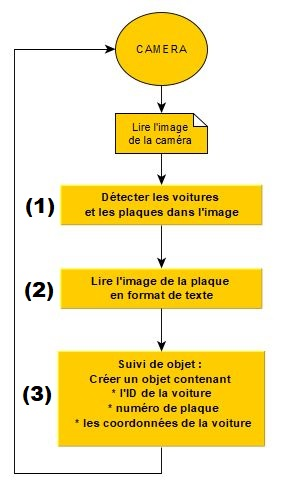
\includegraphics[height=05cm]{ch4-Simple_system_diagram.jpg}
	\caption{Système proposé de gestion de parking intelligent}
 \label{fig:ch4_Simple_system_diagram}
\end{figure}
\subsection{Sous-systèmes de détection de véhicules et de plaques d'immatriculations}
Comme mentionné précédemment, ce travail s'appuie sur le modèle "YOLOv8", "SSD" ou "Faster R-CNN" pour la gestion des parkings. Ce processus implique l'identification et la prédiction des véhicules ainsi que des plaques d'immatriculation Algériennes, réparties en deux catégories : véhicules et plaques d’immatriculation.
\\
L'idée est de construire d'abord une base de données de véhicules, puis d'entraîner le modèle et de le tester sur des images. Pour ce faire, les images collectées sont soumises à un prétraitement et à une annotation. Ensuite, un échantillonnage automatique des données est appliqué pour former des ensembles d'images destinés à l'entraînement, à la validation et aux tests.
%(70 \%) des images de données ont été utilisées comme échantillons d'apprentissage.
%(20 \%) des images de données ont été utilisées comme ensembles de validation.
%(10\%) des images de données ont été utilisées comme ensembles de test.

Dans la phase d'apprentissage du modèle adapté, les poids du modèle sont calculés en se basant sur les ensembles de données préparés et les poids pré-entraînés. Une fois que l'apprentissage est terminé, il est nécessaire d'évaluer le modèle utilisé sur des données de test en utilisant les poids d'entraînement. Par conséquent, les véhicules munis de plaques d'immatriculation à détecter seront localisés et prédits.


Après cela, l'algorithme et le modèle appropriés sont sélectionnés pour effectuer la tâche de détection de la voiture et de la plaque d'immatriculation sur la base des résultats obtenus.

\subsection{ Sous-système destiné à la reconnaissance des numéros de la plaque d'immatriculation}\label{sec:ocr_by_object_detection}

Après la détection de la voiture et de la plaque d'immatriculation dans l'image, le système extrait la zone correspondante de la plaque d'immatriculation de l'image détectée. Cette zone est utilisée pour créer une nouvelle image. Ensuite, le modèle de détection formé sur les numéros de plaque d'immatriculation entre en jeu pour reconnaître les caractères alphanumériques en utilisant les mêmes étapes que dans le système de détection de voiture et de plaque d'immatriculation, à savoir l'échantillonnage, la formation, le test et la vérification de la validité.

La liste des numéros détectés est ensuite organisée dans l'ordre de leur position dans l'image, de gauche à droite, afin de former une chaîne de caractères avec ces numéros, comme illustré dans la figure \ref{fig:ch4-Ocr_my_001}.
\begin{figure}[H]
	\centering
	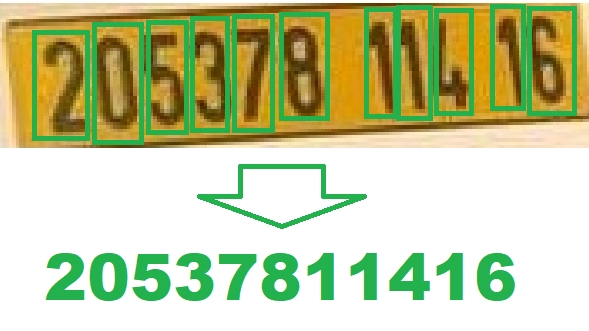
\includegraphics[height=05cm]{ch4-Ocr_my_001.jpg}
	\caption{ Reconnaissance des numéros de la plaque d'immatriculation}
    \label{fig:ch4-Ocr_my_001}
\end{figure}

\subsection{Sous-systèmes de suivi et de comptage en temps réel des véhicules}\label{sec:traking}


Les véhicules identifiés sont exploités dans le processus de suivi et de comptage des véhicules au sein d'une séquence vidéo. Cette séquence enregistre des images de véhicules capturées à des moments successifs. Par conséquent, lorsqu'un véhicule est observé en mouvement dans une vidéo, cela implique que le véhicule occupe une position différente à chaque image consécutive de la vidéo.
\\
L'idée fondamentale derrière le suivi d'objets réside dans la création d'un traqueur d'objet pour chaque objet détecté, afin de suivre son déplacement. Ce suivi se prolonge jusqu'à ce que la N-ième image de la séquence soit atteinte, avec un processus de détection d'objets en cours. Le traqueur d'objets est responsable de la surveillance continue de chaque véhicule, attribuant et maintenant des numéros d'identification (ID) pour chacun.

Dans la phase de suivi de notre système, nous avons mis en œuvre un algorithme simple de suivi d'objets qui se base sur le suivi des centroïdes des objets. Il fonctionne en calculant la distance Euclidienne entre les centroïdes des véhicules déjà existants (c'est-à-dire les véhicules précédemment suivis par le traqueur de centroïdes) et les centroïdes des nouveaux véhicules présents dans les images suivantes de la vidéo. Les étapes complètes de cette solution sont détaillées comme suit :

%Ces étapes sont répétées tout le temps tant que le programme est en cours d'exécution 
\begin{outline}[enumerate]
    \1  Lire un image de la vidéo (ou d'un flux de données en temps réel)à un moment t.
    
    \1  Détecter les véhicules présents dans l'image (en estimant les coordonnées des boîtes englobantes) concernée.
    
    \1  Attribuer un identifiant à chaque véhicule détecté.
    
    \1  Calculer les centroïdes des voitures détectées et les enregistrer dans une liste. 
    
    \1  Lire un nouvelle image de la vidéo à un moment t+1.
    
    \1  Détecter les véhicules présents dans la nouvelle image (en estimant les coordonnées des nouvelles boîtes englobantes).
    
    \1  Calculer la distance entre les centroïdes des nouveaux véhicules et tous les centroïdes d'objets enregistrés dans la liste précédente.Si la distance entre le centre du nouveau véhicule et l'un des centres de la liste est inférieure à une distance minimale prédéfinie, alors le véhicule détecté est considéré comme étant le même que celui déjà enregistré. Le centroïde nouvellement calculé remplace l'ancien centroïde, et l'identifiant reste inchangé. Si la distance entre le centroïde du nouveau véhicule et tous les centres enregistrés dans la liste précédente est supérieure à la distance minimale, alors ce véhicule est considéré comme un nouveau véhicule dans la vidéo. Son centroïde est ajouté à la liste des centroïde avec un nouvel identifiant.
\end{outline}

Si nous divisons la scène sous surveillance de la caméra de sécurité en deux zones,  à savoir la zone B près de la porte du parking et la zone A plus éloignée de la porte du parking, comme illustré dans la figure \ref{ch4-comptage}, il devient possible de compter les véhicules entrants et sortants en suivant le mouvement des véhicules entre les deux zones de la manière suivante :\\
Lorsque nous suivons les véhicules qui se déplacent de la zone A vers la zone B, nous les comptons et les considérons comme le nombre de véhicules entrant dans le parking.\\
Lorsque nous suivons les véhicules qui se déplacent de la zone B vers la zone A, nous les comptons et les considérons comme le nombre de véhicules sortant du parking.

\begin{figure}[H]
	\centering
	\includegraphics[height=05cm]{ch4-comptage.jpg}
	\caption{ Comptage des véhicules}
    \label{ch4-comptage}
\end{figure}

\section{Étude expérimentale}

Les expériences réalisées dans cette section ont été effectuées en utilisant le langage de programmation Python sur la plateforme Google Colaboratory (communément appelée Colab). Cette plateforme utilise l'environnement "Jupyter" (exécuté dans le cloud de Google) pour des tâches d'apprentissage profond et des applications centrées sur les unités de traitement graphique (GPU). En plus de sa facilité d'utilisation (aucune installation préalable requise), Colab offre des ressources de calcul gratuites et prend en charge le développement collaboratif. Du point de vue technique, elle est équipée de 12,8 Go de mémoire vive (RAM) et d'une unité de traitement graphique gratuite (NVIDIA Tesla t4 + 16GB RAM) pouvant être utilisée en continu pendant 12 heures, avec la possibilité d'accéder à d'autres unités de traitement moyennant un abonnement payant. En complément, nous avons utilisé un ordinateur portable équipé d'un processeur \{Intel i5-8350U à 1,70 GHz\}, avec une carte graphique \{Intel UHD Graphics 620\}, sous Windows 10  pour réaliser nos expériences.
Le framework Pytorch est également employé pour construire notre modèle d'apprentissage profond pour la gestion de parking. 

\subsection{Description des jeux de données}

L'initiation du processus de gestion de parking implique la collecte de données d'images. Toutefois, il est ardu de trouver un ensemble de données spécialement conçu pour détecter les véhicules avec des plaques d'immatriculation Algériennes. De surcroît, cet ensemble d'images doit être suffisamment vaste, préserver les détails et bénéficier d'une qualité élevée. En réalité, un tel ensemble de données n'est pas encore disponible.

Dans le cadre de ce travail, nous élaborons notre propre ensemble de données ce qui garantit que les algorithmes de détection ainsi que la reconnaissance peuvent gérer les scénarios et les contextes typiques de l'environnement de gestion de parking de véhicules Algériens.
Dans la section actuelle, nous décrivons le processus de préparation des jeux de données générés, qui visent à: 

\begin{itemize}
\item (1) Détecter les véhicules et les plaques d'immatriculation.
\item (2) Reconnaître les caractères optiques.
\end{itemize}

% ++++++++++++++++++++++++++++++++++++++++++++++++++++++++++++++++++++++++++++++++++++++++++ car

\subsubsection {(1) Jeu de données destiné pour la détection des véhicules et des plaques d'immatriculation Algériennes}


% ++++++++++++++++++++++++++++++++++++++++++++++++++++++++++++++++++++++++++++++++++++++++++ car Collecte d'images

\textbf{Collecte d'images}

Les images ont été rassemblées à partir de deux sources principales :
\begin{itemize}
    \item [$\bullet$] Ouedkniss : un site spécialisé dans la vente d'articles neufs et d'occasion. Ce site abonde en photos de voitures Algériennes proposées à la vente. Pour ce faire, nous avons développé un script Python qui explore le site Ouedkniss, détecte les annonces de voitures et enregistre automatiquement les images dans un fichier.
    
    \item [$\bullet$] Facebook : une plateforme de médias sociaux offrant divers services. Parmi ces services, nous avons exploité la possibilité de collecter un grand nombre de photos de voitures mises en vente. Le téléchargement de ces photos a été effectué manuellement.
    
\end{itemize}
Au total, près de 5000 images ont été collectées à partir de ces deux sources.

% ++++++++++++++++++++++++++++++++++++++++++++++++++++++++++++++++++++++++++++++++++++++++++ car Pré-traitement

\textbf{Pré-traitement des images}

Étant donné que l'ensemble de données que nous avons collecté contient de nombreuses images de mauvaise qualité, nous avons exclu 2620 de ces images. En conséquence, le nombre final d'images est passé à 2380.

% ++++++++++++++++++++++++++++++++++++++++++++++++++++++++++++++++++++++++++++++++++++++++++ car Annotation

\textbf{Annotation des données}

L'annotation manuelle est une tâche extrêmement exigeante, c'est pourquoi il est souvent préférable d'utiliser des outils qui simplifient le processus. Plusieurs options sont disponibles parmi ces outils, dont Roboflow et labelme. Cependant, après une utilisation prolongée de ces deux outils, nous avons rencontré plusieurs problèmes :
\begin{outline}
    \1  Annotation par Roboflow : bien qu'il s'agisse d'un site web, son utilisation a ralenti considérablement le processus d'annotation, en particulier lorsque nous avions un grand nombre d'images à annoter.
    \1 Annotation par labelme : c'est un outil qui s'installe via la ligne de commande Python, mais il a présenté de nombreuses erreurs de programmation. Même après avoir résolu ces erreurs, divers problèmes sont apparus de manière sporadique.
\end{outline}

Nous avons développé notre propre programme qui effectue le processus d'annotation manuel et automatique afin d'affiner les modèles de détection d'objets dans les images. Une fois le développement achevé, nous avons créé une interface graphique en utilisant la bibliothèque PyQt, comme le montre la figure \ref{fig:ch4-yolo_labling_car}.

\begin{figure}[H]
	\centering
	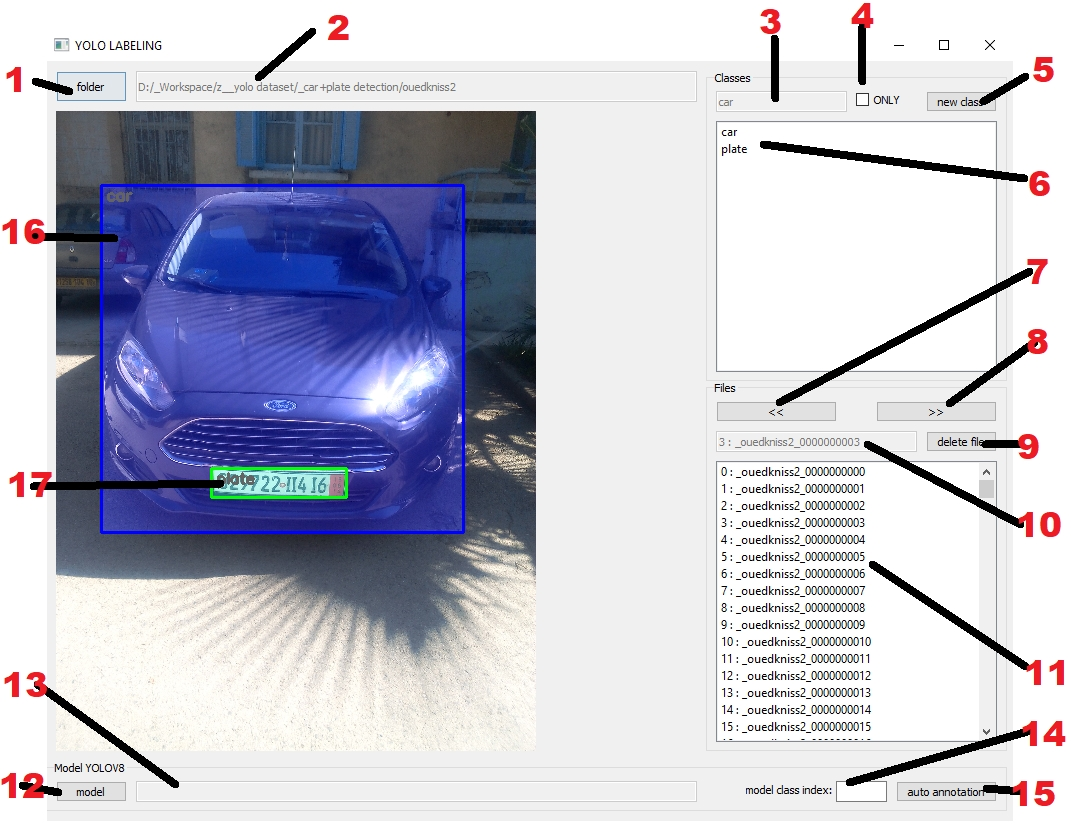
\includegraphics[height=12cm]{ch4-Yolov8_labling.jpg}
	\caption{Annotation des images}
 \label{fig:ch4-yolo_labling_car}
\end{figure}

Sachant que:
\begin{outline}

    \1 1 :  Ce bouton permet de choisir le dossier de travail contenant les images que nous souhaitons utiliser pour générer des étiquettes ("voiture" et "plaque d'immatriculation") et former un modèle de détection d'objet.
    
    \1 2 : Le chemin du dossier de travail actuellement sélectionné s'affiche ici.
    
    \1 3 : Nous pouvons sélectionner la classe d'objet à annoter dans les images. 
    
    
    \1 4 : En sélectionnant un objet dans une image donnée, seuls la boite de délimitation correspondant à cette classe seront affichés.
    
    
    \1 5 : Utiliser ce bouton pour créer une nouvelle classe.
    
    \1 6 : Cette liste affiche toutes les classes disponibles dans la base de données.
    
    \1 7 : Ce bouton nous permet de revenir à l'image précédente.
    
    \1 8 : Bouton pour passer à l'image suivante.
    
    \1 9 : Nous pouvons effacer le fichier image actuel et les annotations associées en utilisant ce bouton.
    
    \1 10 : Le chemin de l'image sur laquelle nous travaillons est affiché ici.
    
    \1 11 : Cette liste présente toutes les images présentes dans le dossier de travail.
    
    
    \1 12 : Sélection d'un modèle de détection d'objets pré-entraîné, tel que YOLOv8, pour générer automatiquement des légendes pour les images.
    
    \1 13 : Le chemin du modèle de détection d'objets YOLOv8 pré-entraîné est indiqué ici.
    
    \1 14 : Entrer le numéro de classe que nous souhaitons que le programme détecte dans les images du dossier de travail. Une fois que ses coordonnées sont identifiées dans les images, le programme génère des annotation pour la classe sélectionnée et enregistre.
    
    \1 15 : Ce bouton démarre le processus de génération automatique des étiquettes pour les images. 

\end{outline}
A la fin, le fichier d'annotation sera créé automatiquement avec le même nom que l'image avec une extension txt.

% ++++++++++++++++++++++++++++++++++++++++++++++++++++++++++++++++++++++++++++++++++++++++++ car Échantillonnage

\textbf{Échantillonnage de données}
\par Dans l'échantillonnage de données, nous avons divisé notre premier jeu de données en trois ensembles distincts : un ensemble d'entraînement, un ensemble de validation et un ensemble de test, en respectant les proportions suivantes :

\begin{outline}

\1 70\% (1667 images) de l'ensemble de données est utilisé pour l'entraînement (Training set).

\1 20\% (475 images) de l'ensemble de données est réservé à la validation (Validation set).

\1 10\% (238 images) de l'ensemble de données est dédié aux tests (Testing set).

\end{outline}

Cette approche est courante dans le domaine de l'apprentissage automatique, où le partitionnement se fait comme le montre la figure \ref{fig:split_dataset_car}.

\begin{figure}[H]
	\centering
	\includegraphics[height=02cm]{ch4-split01.jpg}
	\caption{Échantillonnage du jeu de données}
    \label{fig:split_dataset_car}
\end{figure}

% ++++++++++++++++++++++++++++++++++++++++++++++++++++++++++++++++++++++++++++++++++++++++++ car Augmentation 

\textbf{Augmentation du jeu de données}

L'augmentation de données est une technique couramment utilisée dans le domaine de l'apprentissage automatique pour améliorer les performances des modèles prédictifs en fournissant l'avantage de variations de données d'entraînement disponibles. L'idée principale derrière l'augmentation de données est de générer de nouvelles données (d'apprentissage) en appliquant des transformations ou des manipulations aux données (d'apprentissage) d'origine, tout en préservant leur sémantique et leur classe.
Les avantages de l'augmentation de données comprennent :

\begin{outline}
\1 Elle augmente la taille de données d'entraînement disponibles, en réduisant ainsi le risque de sur-ajustement (overfitting) et en améliorant la capacité du modèle à reconnaître de nouveaux motifs et caractéristiques plus robustes.
\1 Elle aide à renforcer la capacité du modèle à traiter les variations dans les données réelles.
\1 De plus, l'augmentation de données réduit la dépendance à l'égard de vastes quantités de données d'entraînement, ce qui permet de créer des modèles performants avec moins de données.
\end{outline}

Le site Roboflow propose de nombreuses méthodes d'augmentation de données, bien que l'option gratuite offre moins de fonctionnalités et de types d'augmentation de données. Nous avons appliqués sur notre ensemble de données ce qui suit et aussi comme le montre la figure \ref{fig:Augmentation_roboflow}:
\\
- Le retournement horizontal, la rotation dans la plage de -5° à +5°.\\
- La déformation horizontale et verticale.\\
- La conversion partielle en niveaux de gris pour environ 25\% des images.\\
- L'ajustement de la teinte dans l'intervalle de -23° à +23°.\\
- La modification de la saturation entre -25\% et +25\%.\\
- La variation de la luminosité entre -25\% et +25\%.\\
- La modification de l'exposition dans la plage de -25\% à +25\%.\\
- Le flou jusqu'à 1.25 pixel et l'ajout de bruit jusqu'à 1 pixel.\\

\begin{figure}[H]
	\centering
	\includegraphics[height=07cm]{ch4-augmontation.jpg}
	\caption{Méthodes d'augmentation de données}
    \label{fig:Augmentation_roboflow}
\end{figure}

Après avoir réalisé l'augmentation de données sur l'ensemble d'entraînement,  après qu'elles étaient de 1667, elles sont devenues 5001, alors que nous n'avons pas modifié les données testing et de validation , Les résultats étaient les suivants et comme le montre la figure \ref{fig:Aug}.

Après avoir appliqué l'augmentation de données à l'ensemble d'entraînement, qui est passé de 1667 à 5001 images, nous n'avons pas apporté de modifications aux ensembles de données de test et de validation. Les résultats obtenus sont résumés comme suit:\\
- 88 \% (5001 images) des images de données ont été utilisées comme échantillons d'apprentissage.\\ 
- 8 \% (474 image ) des images de données ont été utilisées comme ensembles de validation.\\ 
- 4 \% (238 images ) des images de données ont été utilisées comme ensembles de test.

\begin{figure}[H]
	\centering
	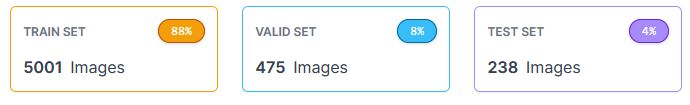
\includegraphics[height=02cm]{img/ch4-Augmentation_car+plate.jpg}
	\caption{Augmentation du jeu de données}
 \label{fig:Aug}
\end{figure}

Une fois que nous avons terminé, nous avons rendu la base de données publique et disponible pour usage en la publiant sur le site web Roboflow à l'adresse suivante : \url{https://universe.roboflow.com/lounisamr/car-plate-dzex/dataset/2}.

%Augmentation du jeu de données


% ++++++++++++++++++++++++++++++++++++++++++++++++++++++++++++++++++++++++++++++++++++++++++ OCR 


\subsubsection {(2) Jeu de données destiné pour la reconnaissance des numéros d'immatriculation }

Pour ce qui est de l'ensemble de données prévu pour la reconnaissance des caractères optiques, nous avons adopté les mêmes étapes que celles utilisées pour l'ensemble de données dédié à la détection des véhicules et des plaques d'immatriculation.

 % ++++++++++++++++++++++++++++++++++++++++++++++++++++++++++++++++++++++++++++++++++++++++++ OCR  Collecte d'images
 
\textbf{Collecte d'images}

Nous avons d'abord développé un script Python qui est capable de lire les images annotées ainsi que leurs fichiers d'annotation associés à partir du premier jeu de données. 
Ensuite, ce script extrait la région qui correspond à la plaque d'immatriculation, la découpe et la sauvegarde en tant que nouvelle image. Le jeu de données ainsi crée comprend un ensemble varié d'images contenant les plaques d'immatriculation Algériennes. L'objectif est de construire un nouveau jeu de données spécifiquement orienté vers la reconnaissance des caractères optiques.

\begin{figure}[H]
	\centering
	\includegraphics[height=07cm]{ch4-crop_plate_001.jpg}
	\caption{Extraction des plaques d'immatriculation.}
    \label{fig:CropPlate}
\end{figure}

 % ++++++++++++++++++++++++++++++++++++++++++++++++++++++++++++++++++++++++++++++++++++++++++ OCR  Pré-traitement
 
\textbf{Pré-traitement des images}

\par Après avoir créé les images de plaques d’immatriculation, nous avons constaté que la majorité de ces images présentaient des problèmes de qualité. Par conséquent, nous effectuons un processus de tri pour ne conserver que les images de la plus haute qualité. C'est pourquoi nous avons développé un script Python qui parcourt toutes les images et supprime celles qui font moins de 200 pixels de large. Ce processus a abouti à un total de 626 images. Ensuite, nous supprimons les photos qui ne répondent pas à nos normes de qualité. A l’issue de cette étape, nous avons pu constituer une collection finale de 417 images de plaques d’immatriculation algériennes de haute qualité.

 % ++++++++++++++++++++++++++++++++++++++++++++++++++++++++++++++++++++++++++++++++++++++++++ OCR  Annotation
 
\textbf{Annotation des numéros d'immatriculation }

\par Pour ajouter des annotations aux caractères sur les images des plaques d'immatriculation en vue de leur identification, nous avons employé le même programme que celui que nous avions précédemment développé pour annoter les voitures et les plaques d'immatriculation.

De cette manière, nous avons généré des boîtes de délimitation autour de chaque numéro de la plaque d'immatriculation et leur avons assigné les étiquettes correspondantes ([0, 1, 2, 3, 4, 5, 6, 7, 8, 9]), comme illustré dans la figure \ref{fig:ch4-annotation_ocr}. Nous avons également préservé les fichiers d'annotations associés à ces numéros de plaques.

\begin{figure}[H]
	\centering
	\includegraphics[height=10cm]{ch4-annotation_ocr.JPG}
	\caption{Annotation des numéros d'immatriculation}
    \label{fig:ch4-annotation_ocr}
\end{figure}


 % ++++++++++++++++++++++++++++++++++++++++++++++++++++++++++++++++++++++++++++++++++++++++++ OCR  Échantillonnage
 
\textbf{Échantillonnage du jeu de données}
\par Nous avons maintenu les mêmes ratios que ceux du premier jeu de données : 80\% pour l'ensemble d'entraînement, 20\% pour la validation et 10\% pour les tests, conformément à ce qui est présenté dans la figure \ref{fig:ch4-divis-ocr-p1}.

\begin{outline}

\1 71\% (330 images) de l'ensemble de données est utilisé pour l'entraînement (Training set).

\1 19\% (81 images) de l'ensemble de données est réservé à la validation (Validation set).

\1 10\% (41 images) de l'ensemble de données est dédié aux tests (Testing set).

\end{outline}

Cette approche est courante dans le domaine de l'apprentissage automatique, où le partitionnement se fait comme le montre la figure \ref{fig:ch4-divis-ocr-p1}.

\begin{figure}[H]
	\centering
	\includegraphics[height=03cm]{ch4-divis-ocr-p1.jpg}
	\caption{Échantillonnage du jeu de données.}
\label{fig:ch4-divis-ocr-p1}
\end{figure}

 % ++++++++++++++++++++++++++++++++++++++++++++++++++++++++++++++++++++++++++++++++++++++++++ OCR  Augmentation
 
\textbf{Augmentation de données}

Nous avons appliqué les mêmes techniques d'augmentation de données à l'ensemble d'entraînement,comme le montre la figure \ref{fig:Augmentation_roboflow}.

Suite à l'augmentation de données sur l'ensemble d'entraînement, qui est passé de 303 à 909 échantillons, alors que les données de test et de validation sont restées inchangées. Les résultats obtenus sont présentés dans la figure \ref{fig:ch4-divis-ocr-p2}, où :\\
- 88 \% (909 images) des images de données ont été utilisées comme échantillons d'apprentissage.\\ 
- 8 \% (81 image ) des images de données ont été utilisées comme ensembles de validation. \\
- 4 \% (41 images ) des images de données ont été utilisées comme ensembles de test.
\begin{figure}[H]
	\centering
	\includegraphics[height=03cm]{ch4-divis-ocr-p2.jpg}
	\caption{Augmentation du jeu de données}
\label{fig:ch4-divis-ocr-p2}
\end{figure}

Nous avons également mis la base de données à disposition du public via le lien suivant : \url{https://universe.roboflow.com/lounisamr/ocr-dz/dataset/2}.


\subsection{Configuration des hyperparamètres}
Afin d'obtenir les meilleurs résultats en matière de détection de véhicules et de plaques d'immatriculation, ainsi que de reconnaissance de numéros de plaques d'immatriculation, nous avons effectué des tests expérimentaux approfondis pour ajuster les hyperparamètres de YOLOV8n, YOLOV8s, YOLOV8m, SSDLITE320 MOBILENETv3 (SSD) et FASTERRCNN MOBILENETv3 (Faster RCNN).
\par Le tableau \ref{table:hyperparamètres} affiche les différentes valeurs des hyperparamètres utilisés dans ces modèles.

\begin{table}[H]
	\centering
	\caption{ Configuration des hyperparamètres }
    \label{table:hyperparamètres}
	\begin{tabular}{|l|l|}
	\hline
	Hyperparamètres & Valeurs  \\
	\hline
	Batch size          & 16  \\
	Epoques              & 10 - 100\\
	Optimizer			& Adam\\
	Taux d'apprentissage       & Changer la valeur par défaut pendant l'apprentissage \\
	Shuffle             & True Train et Faux tests et validation \\
	Fonction d'activation &  Softmax  et Relu \\
       Taille d'image & 224, 320, 416, 512, 640 \\
	\hline  
	\end{tabular}%
\end{table}


%appliquant les mêmes paramètres et la même base de données afin de choisir le meilleur modèle pour servir de base au programme de gestion du stationnement, et les critères les plus importants sur lesquels se concentreront sont la vitesse du modèle à détecter les objets dans les images et la précision de la détection.

\subsection{Entraînement du modèle YoloV8}
% +++++++++++++++++++++++++++++++++++++++++++++++++++++++++++++++++++ YOLOV8 CAR
\subsubsection{Entraînement de modèle YOLOV8n pour la détection de voitures et de plaques}

L'entraînement d'un modèle YOLOv8 pour la détection de deux classes, à savoir les voitures et les plaques d'immatriculation, a été initié en utilisant un modèle pré-entraîné sur le jeu de données COCO, comprenant 80 catégories. Le processus a impliqué une technique de transfert d'apprentissage pour adapter le modèle en ajustant des paramètres tels que la taille de l'image d'entrée (320x320) et la taille de la sortie \{boite de délimitation, classe, scores de prédiction\}, tout en conservant les poids existants. L'algorithme YOLO est caractérisé par trois fonctions de perte : "cls loss", dfl loss" et "box loss". La première fonction mesure l'erreur ou la divergence entre les prédictions du modèle concernant la classe d'objets. La seconde fonction mesure l'erreur ou la divergence entre les prédictions du modèle concernant le flou ou la netteté (focus) des objets dans les boîtes englobantes et les véritables niveaux de flou des objets. En d'autres termes, elle évalue à quel point le modèle est précis pour déterminer si un objet est net ou flou dans l'image. La dernière fonction mesure l'erreur ou la divergence entre les prédictions du modèle concernant les coordonnées des boîtes englobantes.

Les figures \ref{fig:ch4-yolov8n_car_loss} et \ref{fig:ch4-yolov8n_car_mAP} présentent, respectivement, les courbes de perte associées à ces trois fonctions et les graphes de mAPs, de précision et de rappel.

%%%%%%%  dans la phase du test: Résultats et discussion:%%%%%%%%%%%%%%%%%%%%%%%%%%%%%%%%%%%%%%%%%%%%%%%%




\begin{figure}[H]
	\centering
	\includegraphics[height=04.5cm]{ch4-yolov8n_car_loss.jpg}
	\caption{Courbes de pertes du YOLOV8n pour la détection de voitures et de plaques }
\label{fig:ch4-yolov8n_car_loss}
\end{figure}

\begin{figure}[H]
	\centering
	\includegraphics[height=04.5cm]{ch4-yolov8n_car_mAP.jpg}
	\caption{Courbes de mAPs, de précision et de rappel du YOLOV8n pour la détection de voitures et de plaques}
\label{fig:ch4-yolov8n_car_mAP}
\end{figure}

Nous observons que les trois courbes de perte générées par le modèle YOLOv8n pendant l'apprentissage montrent une convergence lente mais stable, nécessitant environ 25 itérations pour atteindre une valeur de perte (train/cls\_loss) de prédictions des classes d'objet d'environ 0,35 pour et une valeur de perte (train/box\_loss) approximative de 0.55  pour les prédictions des coordonnées des boites de délimitation.\\
Comparativement aux courbes instables de mAP, de précision et de rappel, le modèle atteint sa convergence lors de la 25ème itération. À ce stade, les valeurs de mAP sont supérieures à 99,4\%, la précision dépasse les 99,5\%, et le rappel atteignait 98,8\%.


% +++++++++++++++++++++++++++++++++++++++++++++++++++++++++++++++++++ YOLOV8 OCR
\subsubsection{Entraînement du modèle YOLOV8n pour la reconnaissance des chiffres}

Lors de l'entraînement du modèle YOLOv8 pour la reconnaissance des chiffres d'immatriculation \{0, 1, 2, 3, 4, 5, 6, 7, 8, 9 \}, nous appliquons le même principe cité précédemment (apprentissage par transfert).

Les figures \ref{fig:ch4-yolov8n_ocr_loss} et \ref{fig:ch4-yolov8n_ocr_amp} illustrent respectivement les courbes de perte associées et les graphes de mAPs, de précision et de rappel du modèle YOLOV8n pour la reconnaissance des chiffres d'immatriculation.

\begin{figure}[H]
	\centering
	\includegraphics[height=04.5cm]{ch4-yolov8n_ocr_loss.jpg}
	\caption{Courbes de pertes du YOLOV8n pour la reconnaissance des chiffres}
\label{fig:ch4-yolov8n_ocr_loss}
\end{figure}

\begin{figure}[H]
	\centering
	\includegraphics[height=04.5cm]{ch4-yolov8n_ocr_mAP.jpg}
	\caption{Courbes de mAPs du YOLOV8n pour la reconnaissance des chiffres}
\label{fig:ch4-yolov8n_ocr_amp}
\end{figure}

% \textcolor{blue}{Il faut commenter }
%Nous observons que les trois courbes de perte générées par le modèle YOLOv8n pendant l'apprentissage montrent une convergence lente mais stable, nécessitant environ 80 itérations pour atteindre une valeur de perte (train/cls\_loss) de prédictions des classes d'objet d'environ 0,35 pour et une valeur de perte (train/box\_loss) approximative de 0.80  pour les prédictions des coordonnées des boites de délimitation.\\
%Comparativement aux courbes instables de mAP, de précision et de rappel, le modèle atteint sa convergence lors de la 80ème itération. À ce stade, les valeurs de mAP sont supérieures à 99,4\%, la précision dépasse les 99,5\%, et le rappel atteignait 98,8\% .

Lors de l'apprentissage du modèle YOLOv8n, on note que les courbes de perte montrent une convergence lente mais stable, nécessitant environ 80 itérations pour atteindre des valeurs de perte de 0,4 pour les prédictions de classes (\textit{train/cls\_loss})  d'objets et de 0,80 pour les prédictions de coordonnées (\textit{train/box\_loss}) de boîtes de délimitation. En revanche, les courbes de performance telles que mAP, précision et rappel convergent beaucoup plus rapidement, dès la 10ème itération, avec des valeurs de mAP supérieures à 99,4\%, une précision dépassant 99,5\%, et un rappel atteignant 98,8\%.

% +++++++++++++++++++++++++++++++++++++++++++++++++++++++++++++++++++ Faster R-CNN CAR
\subsection{Entraînement du modèle Faster R-CNN}
Pour le modèle FASTERRCNN\_MOBILENET\_V3\_LARGE\_FPN, nous avons suivi des étapes d'entraînement similaires à celles que nous avons utilisées pour le modèle YOLOv8.

\subsubsection{Entraînement du modèle Faster R-CNN pour la détection des voitures et des plaques d'immatriculation}

Les figures \ref{fig:ch4-frcnn-car_loss} et \ref{fig:ch4-frcnn-car_mAP}démontrent, respectivement, les graphes de pertes, y compris les pertes de classification "loss\_classifier", de régression de boîte "loss\_box\_reg", d'objectness "loss\_objectness", et de régression de boîte RPN "loss\_rpn\_box\_reg\" du modèle ainsi que les graphiques de la mAP pour le modèle Faster R-CNN.


\begin{figure}[H]
	\centering
	\includegraphics[height=04.5cm]{ch4-frcnn-car_loss.jpg}
	\caption{Courbes de pertes du Faster R-CNN pour la détection de voitures et de plaques }
\label{fig:ch4-frcnn-car_loss}
\end{figure}

\begin{figure}[H]
	\centering
	\includegraphics[height=04.5cm]{ch4-frcnn-car_mAP.jpg}
	\caption{Courbes de mAPs du Faster R-CNN pour la détection de voitures et de plaques}
\label{fig:ch4-frcnn-car_mAP}
\end{figure}

% \textcolor{blue}{Il faut commenter }
Lors de l'apprentissage du modèle Faster R-CNN, nous remarquons que les courbes de perte convergent rapidement, bien qu'elles présentent des fluctuations. Il faut environ 7 itérations pour que la perte liée à la classification des d'objets (loss\_classifier)  atteigne environ 0,03, et la perte associée à la régression (loss\_box\_reg) des prédictions de coordonnées des boîtes de délimitation atteigne environ 0,180.\\
En ce qui concerne les courbes de performance, telles que mAP50 (moyenne des précisions pour un seuil de confiance de 50\%) et mAP75 (moyenne des précisions pour un seuil de confiance de 75\%), elles sont également instables, mais le modèle atteint une convergence avec des valeurs dépassant respectivement 96\% et 86\% dès la 10ème itération.


% +++++++++++++++++++++++++++++++++++++++++++++++++++++++++++++++++++ Faster R-CNN OCR
\subsubsection{Entraînement du modèle Faster R-CNN pour la reconnaissance des numéros d'immatriculation}

Les figures \ref{fig:ch4-frcnn_ocr_loss} et \ref{fig:ch4-frcnn_ocr_mAP} présentent, respectivement, les courbes de perte, y compris les pertes de classification, de régression de boîte, de objectness, et de régression de boîte RPN, ainsi que les graphiques de la mAP pour le modèle Faster R-CNN.


\begin{figure}[H]
	\centering
	\includegraphics[height=04.5cm]{ch4-frcnn_ocr_loss.jpg}
	\caption{Courbes de pertes du Faster R-CNN pour la reconnaissance des chiffres}
\label{fig:ch4-frcnn_ocr_loss}
\end{figure}

\begin{figure}[H]
	\centering
	\includegraphics[height=04.5cm]{ch4-frcnn_ocr_mAP.jpg}
	\caption{Courbes de mAps du Faster R-CNN pour la reconnaissance des chiffres}
\label{fig:ch4-frcnn_ocr_mAP}
\end{figure}

% \textcolor{blue}{Il faut commenter le tableau, quel est le meilleur modèle selon vous, votre interprétation n'est pas complete}

% \textcolor{blue}{Il faut commenter }

%Nous observons que les quatre courbes de perte générées par le modèle Faster R-CNN pendant l'apprentissage montrent une convergence rapide, nécessitant environ 15 itérations 
%pour atteindre une valeur de perte (loss\_classifier) de prédictions des classes d'objet d'environ 0,1 
%pour et une valeur de perte (loss\_box\_reg) approximative de 0.4 pour les prédictions des coordonnées des boites de délimitation.\\
%Comparativement aux courbes de mAP50 et mAP75 d le modèle atteint sa convergence lors de la 15ème itération.À ce stade, les valeurs de mAP50 sont supérieures à 96\%, la mAP75 dépasse les 86\%.


Il est noté que les quatre courbes de perte générées par le modèle Faster R-CNN pendant l'apprentissage montrent une convergence rapide. Il faut environ 6 itérations pour que la perte associée à la classification des classes d'objet (\textit{loss\_classifier}) atteigne environ 0,1, tandis que la perte liée à la régression des coordonnées des boîtes de délimitation (\textit{loss\_box\_reg}) soit 0,38.

En comparaison avec les courbes de mAP50 et mAP75, le modèle atteint une convergence dès la 6ème itération. À ce stade, les valeurs de mAP50 dépassent les 96\%, tandis que la mAP75 dépasse les 86\%.

 
% +++++++++++++++++++++++++++++++++++++++++++++++++++++++++++++++++++ SSD CAR
\subsection{Entraînement du modèle SSD}
\subsubsection{ Entraînement du modèle SSD pour la détection des voitures et des plaques d'immatriculation}

Les figures \ref{fig:ch4-ssd car loss} et \ref{fig:ch4-ssd car mAP} présentent, respectivement, les courbes de perte, y compris les pertes de classification, de régression de boîte, de objectness, et de régression de boîte RPN, ainsi que les graphiques de la mAP pour le modèle SSDLite320\_MOBILENET\_V3\_LARGE.


\begin{figure}[H]
	\centering
	\includegraphics[height=04.5cm]{ch4-ssd car loss.jpg}
	\caption{Courbes de pertes du SSD pour la détection de voitures et de plaques}
\label{fig:ch4-ssd car loss}
\end{figure}


\begin{figure}[H]
	\centering
	\includegraphics[height=04.5cm]{ch4-ssd car mAP.jpg}
	\caption{Courbes de mAPs du SSD pour la détection de voitures et de plaques}
\label{fig:ch4-ssd car mAP}
\end{figure}

% \textcolor{blue}{Il faut commenter le tableau, quel est le meilleur modèle selon vous, votre interprétation n'est pas complete}

Le modèle SSD montre une convergence rapide de ses courbes de perte, nécessitant environ 8 itérations pour atteindre une perte de classification d'environ 0,5 et une perte de régression d'environ 0,05 pour les boîtes de délimitation. En ce qui concerne la moyenne de la précision moyenne, le modèle atteint sa convergence dès la 8ème itération, avec une mAP50 dépassant 80\% et une mAP75 dépassant 90\%.

% +++++++++++++++++++++++++++++++++++++++++++++++++++++++++++++++++++ SSD OCR
\subsubsection{Entraînement du modèle SSD pour la reconnaissance des numéros d'immatriculation}

Les figures \ref{fig:ch4-SSD ocr loss} et \ref{fig:ch4-SSD ocr mAP} présentent, respectivement, les courbes de perte, y compris les pertes de classification, de régression de boîte, de objectness, et de régression de boîte RPN, ainsi que les graphiques de la mAP pour le modèle Faster R-CNN.


\begin{figure}[H]
	\centering
	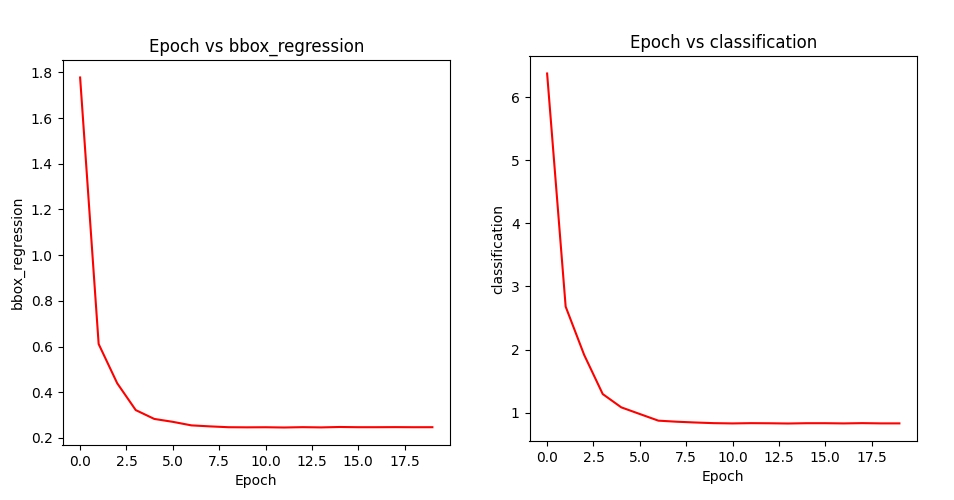
\includegraphics[height=05cm]{ch4-SSD ocr loss.jpg}
	\caption{Courbes de pertes du SSD pour la reconnaissance des chiffres}
\label{fig:ch4-SSD ocr loss}
\end{figure}

\begin{figure}[H]
	\centering
	\includegraphics[height=05cm]{ch4-SSD ocr mAP.jpg}
	\caption{Courbes de mAPs du SSD pour la reconnaissance des chiffres}
\label{fig:ch4-SSD ocr mAP}
\end{figure}

% \textcolor{blue}{Il faut commenter }
%Nous observons que les deux  courbes de perte générées par le modèle SSD pendant l'apprentissage montrent une convergence rapide, nécessitant environ 8 itérations 
%pour atteindre une valeur de perte (loss\_classifier) de prédictions des classes d'objet d'environ 0,5
%pour et une valeur de perte (loss\_box\_reg) approximative de 0.3 pour les prédictions des coordonnées des boites de délimitation.\\
%Comparativement aux courbes de mAP50 et mAP75 d le modèle atteint sa convergence lors de la 15ème itération.À ce stade, les valeurs de mAP50 sont supérieures à 65\%, la mAP75 dépasse les 75\%.

Les courbes de perte du modèle SSD pendant l'apprentissage convergent rapidement, atteignant environ 0,5 pour la perte de classification des classes d'objet et environ 0,3 pour la perte de régression des coordonnées des boîtes de délimitation après environ 8 itérations. En ce qui concerne les courbes de mAP50 et mAP75, le modèle atteint sa convergence à la 15ème itération, avec des valeurs de mAP50 dépassant 65\% et mAP75 dépassant 75\%.

\section{Résultats et discussion}

Dans cette section, nous allons évaluer et comparer les performances de cinq modèles de détection : YOLOv8n, YOLOv8m, YOLOv8s, Faster RCNN et SSD. Nous allons examiner leurs performances tant lors de la phase d'apprentissage que lors des tests pour les tâches de détection des voitures, des plaques d'immatriculation, ainsi que pour la reconnaissance des chiffres d'immatriculation.

L'objectif de cette évaluation est de choisir le modèle le plus performant en vue de son déploiement dans une ordinateur et un smartphone.
% +++++++++++++++++++++++++++++++++++++++++++++++++++++++++++++++++++ result CAR
\subsection{Résultats de l'entraînement et du test des modèles de détection de voitures et de plaques d'immatriculation}

Dans la première expérience, nous faisons varier les valeurs de la dimension de l'image d'entrée et du nombre d'époques d'apprentissage. Nous enregistrons ensuite, pour chaque combinaison de valeurs, la moyenne de la précision moyenne (mAP50), la taille du modèle généré (représentant le fichier de poids résultant de l'apprentissage en MB), et le temps d'apprentissage (en minutes) pour la détection de voitures et de plaques d'immatriculation. Ces résultats sont présentés dans le tableau \ref{table:ch4-training_car_allmodels}.

\begin{table}[h]
	\centering
    \begin{tabular}{|l|l|l|l|l|l|}
    \hline
        Modèle & \shortstack{Dimension \\ d'image}  & Epoque &    mAP50 & \shortstack{Taille \\du modèle}   & \shortstack{Temps\\ d'apprentissage } \\ \hline
        \textbf{YOLOv8n} & \textbf{320x320} &      \textbf{25}     & \textbf{0.995} &  \textbf{6} &      \textbf{38}    \\ \hline
        YOLOv8n &  416x416 &     25     & 0.994  & 6 &     44    \\ \hline
        YOLOv8n & 512x512  &     25    & 0.995   &  6 &  54     \\ \hline
        YOLOv8n & 640x640 &      25     &  0.994    &  6 &   63   \\ \hline
        YOLOv8n & 736x736 &      25     &  0.994  &  6 &       81    \\ \hline
        YOLOv8s & 320x320 &      20      & 0.995  &   6 &     33     \\ \hline
        YOLOv8s & 416x416&       20      & 0.994 &  6 &      38    \\ \hline
        YOLOv8s & 512x512 &       20     &   0.995  &     6 &      48   \\ \hline
        YOLOv8s &  640x640&        20     &  0.995 & 6 &      67     \\ \hline
        YOLOv8s & 736x736  &       20     &   0.995 &   6 &       77   \\ \hline
        YOLOv8m & 320x320  &        20   &  0.996  & 50 &     87     \\ \hline
        SSD     & 320x320  &         10   &  0.984    &   9  &   15   \\ \hline
        Faster R-CNN & 320x320   &   10    &  0.99  &  74 &  17     \\ \hline
    \end{tabular}
    \caption{Performances d'entraînement des modèles de détection de voitures et de plaques}
    \label{table:ch4-training_car_allmodels}
\end{table}
% \textcolor{blue}{A vérifier}
D'après le tableau\ref{table:ch4-training_car_allmodels}, nous observons ce qui suit:\\
- YOLOv8n et YOLOv8s : Ces modèles YOLOv8n et YOLOv8s montrent une performance élevée (mAP50 autour de 0,995) sur différentes dimensions d'images, ce qui indique une capacité de détection précise des objets. Les temps d'apprentissage varient en fonction de la taille de l'image d'entrée, avec des images plus grandes nécessitant plus de temps.\\
- YOLOv8m : Le modèle YOLOv8m atteint une précision légèrement supérieure (mAP50 de 0,996), mais il nécessite un temps d'apprentissage plus long en raison de sa taille plus importante.\\
- SSD : Le modèle SSD montre une performance légèrement inférieure (mAP50 de 0,984) par rapport aux modèles YOLOv8, mais il s'entraîne plus rapidement.\\
- Faster R-CNN : Faster R-CNN atteint une précision élevée (mAP50 de 0,99), mais il nécessite plus de temps d'apprentissage que SSD en raison de sa complexité.

Dans la second expérience, nous avons évalué la vitesse des cinq modèles de détection en termes du temps d'inférence (MS), ainsi que le nombre d'images par seconde (FPS), en tenant compte de la taille de l'image d'entrée, comme présenté dans le tableau \ref{table:ch4-test_speed_car_allmodels}. 
Notre objectif était de sélectionner le modèle qui offre la vitesse de détection la plus élevée pour les voitures et les plaques d'immatriculation tout en maintenant la plus grande précision possible.

\begin{table}[H]
    \centering
    \begin{tabular}{|l|l|l|l|}
    \hline
        Modèle & Dimension d'image & Temps d'inférence & FPS\\ \hline
        \textbf{YOLOv8n} & \textbf{320x320} & \textbf{71} & \textbf{14.1} \\ \hline
        YOLOv8n & 416x416 & 83 & 12.0 \\ \hline
        YOLOv8n & 512x512 & 125 & 8.0 \\ \hline
        YOLOv8n & 640x640 & 167 & 6.0 \\ \hline
        YOLOv8n & 736x736 & 250 & 4.0 \\ \hline
        YOLOv8s & 320x320 & 143 & 7.0 \\ \hline
        YOLOv8s & 416x416 & 200 & 5.0 \\ \hline
        YOLOv8s & 512x512 & 250 & 4.0 \\ \hline
        YOLOv8s & 640x640 & 333 & 3.0 \\ \hline
        YOLOv8s & 736x736 & 500 & 2.0 \\ \hline
        YOLOv8m & 320x320 & 600 & 1.7 \\ \hline
        SSD & 320x320 & 110 & 9.1 \\ \hline
        Faster R-CNN & 320x320 & 600 & 1.7 \\ \hline
    \end{tabular}
    \caption{Comparaison de vitesse d'inférence des modèles de détection de voitures et de plaques }
    \label{table:ch4-test_speed_car_allmodels}
\end{table}

Nous pouvons remarquer, selon le tableau \ref {table:ch4-test_speed_car_allmodels}, que YOLOv8n  semble être le plus rapide parmi les YOLOv8 variantes avec de bonnes performances. Cependant, à mesure que la dimension de l'image augmente, les performances chutent, ce qui est attendu car le modèle doit traiter une image plus grande. YOLOv8s  est plus rapide que YOLOv8n, mais il a également de moins bonnes performances en termes de FPS. Cependant, il offre une meilleure performance par rapport à YOLOv8n pour les images de plus grande dimension. Bien que YOLOv8m ait de bonnes performances en termes de FPS pour des images de petite dimension, il est nettement moins performant que les autres modèles pour des images plus grandes. SSD offre de bonnes performances en termes de FPS pour des images de petite dimension, mais il est moins performant que les modèles YOLO et Faster R-CNN pour des images de plus grande taille. Faster R-CNN est le modèle le plus lent en termes de FPS, mais il offre une performance constante indépendamment de la dimension de l'image.

En conclusion, nous avons opté pour le modèle YOLOv8n, car il a atteint une vitesse de détection élevée avec une taille d'image de 320x320, tout en conservant une précision élevée, affichant un mAP de 0,995. De plus, il a nécessité un temps d'apprentissage modéré et a généré un modèle de petite taille.

En examinant les figures \ref{fig:ch4-test-yolov8-detection-car}, \ref{fig:ch4-test-frcnn-detection-car} et \ref{fig:ch4-test-ssd-detection-car}, nous pouvons constater que le modèle YOLOv8n a obtenu une très bonne détection de véhicules et de plaques d'immatriculation comparée avec les modèles Faster RCNN et SSD. Les boîtes de délimitation sont correctement localisées autour de tous les objets, avec un bon score de prédiction.

\begin{figure}[H]
	\centering
	\includegraphics[height=4cm]{ch4-test-yolov8-detection-car.jpg}
	\caption{Résultats visuels de la détection de voitures et de plaques par YOLOv8n}
 \label{fig:ch4-test-yolov8-detection-car}
\end{figure}

\begin{figure}[H]
	\centering
	\includegraphics[height=04.5cm]{ch4-test-frcnn-detection-car.jpg}
	\caption{Résultats visuels de la détection de voitures et de plaques par Faster R-CNN}
\label{fig:ch4-test-frcnn-detection-car}
\end{figure}

\begin{figure}[H]
	\centering
	\includegraphics[height=04.5cm]{ch4-test-ssd-detection-car.jpg}
	\caption{Résultats visuels de la détection de voitures et de plaques par SSD}
\label{fig:ch4-test-ssd-detection-car}
\end{figure}



% +++++++++++++++++++++++++++++++++++++++++++++++++++++++++++++++++++ result OCR
\subsection{Résultats de l'entraînement et du test des modèles pour le reconnaissance des chiffres}


De manière similaire, nous avons effectué des expériences pour évaluer la reconnaissance des chiffres d'immatriculation. Les résultats de ces expériences sont résumés dans les tableaux \ref{table:ch4-training_ocr_allmodels} et \ref{table:ch4-test_speed_ocr_allmodels}.

\begin{table}[H]
    \centering
    \begin{tabular}{|l|l|l|l|l|l|}
    \hline
        Modèle & \shortstack{Dimension \\d'image } & Epoque &    mAP50 & \shortstack{Taille \\du modèle}   &  \shortstack{Temps \\ d'apprentissage}     \\ \hline
        YOLOv8n & 96x96          &   80         & 0.93   & 6 & 13  \\ \hline
        YOLOv8n & 128x128         &   80       & 0.986   &  6 &  15\\ \hline
        YOLOv8n & 160x160          &   80       & 0.986   &6  & 16 \\ \hline
        YOLOv8n & 192x192         &    80      & 0.986    &6  & 19 \\ \hline
        \textbf{YOLOv8n} & \textbf{224x224} &\textbf{80}& \textbf{0.994}& \textbf{6} &\textbf{20}\\ \hline
        YOLOv8n &  256x256         &   80     & 0.993    & 6 & 20 \\ \hline
        YOLOv8s & 224x224          &   80      & 0.996   & 21 &  20\\ \hline
        YOLOv8m & 320x320          &    20    & 0.996     & 50  & 22 \\ \hline
        SSD      & 320x320         &   40      & 0.96        & 9 & 10 \\ \hline
        Faster R-CNN & 320x320      & 40        & 0.99    & 74 &  20\\ \hline
    \end{tabular}
    \caption{Entraînement des modèles de pour la reconnaissance des chiffres}
    \label{table:ch4-training_ocr_allmodels}
\end{table}

% \textcolor{blue}{Il faut commenter le tableau, quel est le meilleur modèle selon vous, votre interprétation n'est pas complete} 

Selon le tableau \ref{table:ch4-training_ocr_allmodels}), les valeurs de mAP varient de 0,93 à 0,996. Les modèles YOLOv8n, YOLOv8s et YOLOv8m obtiennent une précision élevée dans la reconnaissance des numéros de plaques d'immatriculation, tandis que SSD affiche une précision légèrement inférieure, et Faster R-CNN atteint également une précision importante.

En ce qui concerne le temps d'apprentissage, les modèles ont des temps d'apprentissage similaires, d'environ 20 minutes, à l'exception de YOLOv8m, qui nécessite légèrement plus de temps, soit 22 minutes, et de SSD, qui est encore plus rapide avec seulement 10 minutes.

\begin{table}[H]
    \centering
    \begin{tabular}{|l|l|l|}
    \hline
        Modèle  & Dimension d'image & Temps d'inférence \\ \hline
        YOLOv8n & 96x96& 10 \\ \hline
        YOLOv8n & 128x128 & 10 \\ \hline
        YOLOv8n & 160x160 & 10 \\ \hline
        YOLOv8n & 192x192 & 10 \\ \hline
        \textbf{YOLOv8n} & \textbf{224x224} & \textbf{20} \\ \hline
        YOLOv8n & 256x256 & 30 \\ \hline
        YOLOv8s & 224x224 & 330 \\ \hline
         YOLOv8m & 320x320 & 600 \\ \hline
        SSD & 320 & 110x110 \\ \hline
        Faster R-CNN & 320x320 & 600 \\ \hline
    \end{tabular}
    \caption{Comparaison de vitesse d'inférence des modèles pour la reconnaissance des chiffres}
    \label{table:ch4-test_speed_ocr_allmodels}
\end{table}
% \textcolor{blue}{Il faut commenter le tableau, quel est le meilleur modèle selon vous, votre interprétation n'est pas complete} 

Selon les résultats numériques obtenus et indiqués dans le tableau \ref{table:ch4-test_speed_ocr_allmodels}), les modèles YOLOv8n, YOLOv8s, YOLOv8m, SSD et Faster R-CNN présentent des temps d'inférence variables en fonction de la taille de l'image en entrée. De plus, il est à noter que le modèle YOLOv8n atteint la meilleure mAP, avec une valeur de 0,994, lorsque la taille de l'image d'entrée est réglée à 224.

En ce qui concerne les résultats visuels, les figures \ref{fig:ch4-test-yolov8-detection-ocr}, \ref{fig:ch4-test-frcnn-detection-ocr} et \ref{fig:ch4-test-frcnn-detection-ocr} fournissent une illustration de la reconnaissance des chiffres d’immatriculation par les modèles YOLOv8n, Faster RCNN et SSD. 
Selon ces figures, nous pouvons observer que les boîtes de délimitation prédites par le modèle YOLOv8n ont été générées de manière précise autour de chaque chiffre présent sur les panneaux numériques, avec un taux de prédiction élevé.Entre ce que Faster R-CNN et SSD ont échoué à reconnaître, il y a quelques différences.

\begin{figure}[H]
	\centering
	\includegraphics[height=05cm]{ch4-test-yolov8-detection-ocr.jpg}
	\caption{Résultats visuels de la reconnaissance des chiffres d'immatriculation par YOLOv8n}
\label{fig:ch4-test-yolov8-detection-ocr}
\end{figure}

\begin{figure}[H]
	\centering
	\includegraphics[height=04.5cm]{ch4-test-frcnn-detection-ocr.jpg}
	\caption{ Résultats visuels de la reconnaissance des chiffres par Faster R-CNN}
\label{fig:ch4-test-frcnn-detection-ocr}
\end{figure}


\begin{figure}[H]
	\centering
	\includegraphics[height=05cm]{ch4-test-ssd-detection-ocr.jpg}
	\caption{Résultats visuels de la reconnaissance des chiffres par SSD}
\label{fig:ch4-test-ssd-detection-ocr}
\end{figure}
% +++++++++++++++++++++++++++++++++++++++++++++++++++++++++++++++++++ Comparaison OCR
\subsection{Application des outils spécialisés pour la reconnaissance des chiffres}

En parallèle, nous avons utilisé d'autres outils spécifiques à la reconnaissance ou à la lecture des chiffres d'immatriculation à partir d'images de plaques d'immatriculation, qui contiennent principalement du texte. Parmi ces outils, nous citons notamment EasyOCR\cite{ch4_EasyOCRsdsdsd}, OpenALPR\cite{openalpr-readme} et Tesseract OCR \cite{tesseract-ocr-guide}, en plus des modèles que nous avons développées, en particulier le modèle YOLOv8n.

\textbf{Tesseract OCR :} est un moteur de reconnaissance optique de caractères open source et gratuit, disponible sous licence Apache. Il est développé par Google depuis 2006\cite{ch4_ocr_Tesserac35}. Il est capable de reconnaître des textes imprimés dans une variété de langues, y compris le français, l'anglais, l'allemand, l'espagnol, le chinois et le japonais. Il peut être utilisé pour extraire des textes de documents scannés, de photos et d'autres images. Tesseract est disponible pour les systèmes d'exploitation Windows, macOS et Linux. Il peut être utilisé via une interface de ligne de commande ou une API.

Comme indiqué dans la figure \ref{fig:ch4-tesseract-ocr}, Tesseract n'a pas réussi à reconnaître correctement les chiffres de la plaque d'immatriculation donnée. De plus, sa vitesse de traitement était extrêmement lente.

\begin{figure}[H]
	\centering
	\includegraphics[height=07cm]{ch4-tesseract-ocr.jpg}
	\caption{Reconnaissance des chiffres d'immatriculation à l'aide du Tesseract}
    \label{fig:ch4-tesseract-ocr}
\end{figure}
\textbf{EasyOCR : } est un outil d'OCR gratuit et facile à utiliser. Il peut être utilisé pour extraire des textes de documents scannés, de photos et d'autres images. EasyOCR prend en charge plus de 100 langues et peut reconnaître une variété de formats de texte \cite{ch4_EasyOCRV83}.

Selon la figure \ref{fig:ch4-easyocr}, EasyOCR n'a pas réussi non plus à lire tous les  chiffre de la plaque d'immatriculation testée.

\begin{figure}[H]
	\centering
	\includegraphics[height=07cm]{ch4-easyocr.jpg}
	\caption{Reconnaissance des chiffres d'immatriculation à l'aide du EasyOCR}
    \label{fig:ch4-easyocr}
\end{figure}

\textbf{OpenALPR :} est un outil spécialisé pour la reconnaissance automatique des plaques d'immatriculation. 
Cependant, ces outils présentent certaines limitations. En effet, ils ne sont pas capables de reconnaître certaines plaques d'immatriculation, comme la plaque d'immatriculation algérienne, sans ajustement préalable des paramètres du pays pour l'analyse des images. De plus, ils sont lents et nécessitent un temps de traitement important.

Conformément à ce qui est illustré dans la figure \ref{fig:ch4-openalpr}, lors de l'utilisation d'OpenALPR sur des plaques d'immatriculation américaines, les chiffres sont correctement reconnus, mais cela demande un temps de traitement de 1840 millisecondes. Cependant, lors de son application sur des plaques algériennes, aucun symbole n'est détecté dans la plaque d'immatriculation algérienne, ce qui a été confirmé dans \cite{ch4_OpenALPR81}.
 
\begin{figure}[H]
	\centering
	\includegraphics[height=07cm]{ch4-openalpr.jpg}
	\caption{Reconnaissance des chiffres d'immatriculation à l'aide du OpenALPR}
    \label{fig:ch4-openalpr}
\end{figure}

\section{Gestion de parking : Application pour les véhicules en Algérie}

Dans le cadre de notre projet de fin d'études, nous avons réalisé une application intelligente spécialement conçue pour gérer efficacement le stationnement des conducteurs de véhicules en Algérie.  
Cette application a été développée pour fonctionner sur un ordinateur portable et offre les fonctionnalités suivantes :
\begin{outline}[enumerate]
    \1 Détection des véhicules et des plaques d'immatriculation,
    \1 Reconnaissance des numéros d'immatriculation,
    \1 Suivi en temps réel des véhicules en analysant les vidéos provenant des caméras de surveillance,
    \1 Comptage des véhicules entrants et sortants du parking et l'enregistrement de la date d'entrée ou de sortie des véhicules.
\end{outline} 
La Figure \ref{fig:final_soft} présente l'interface principale de l'application que nous avons développée, où les régions numérotées sont expliquées comme suit :

\begin{figure}[H]
	\centering
	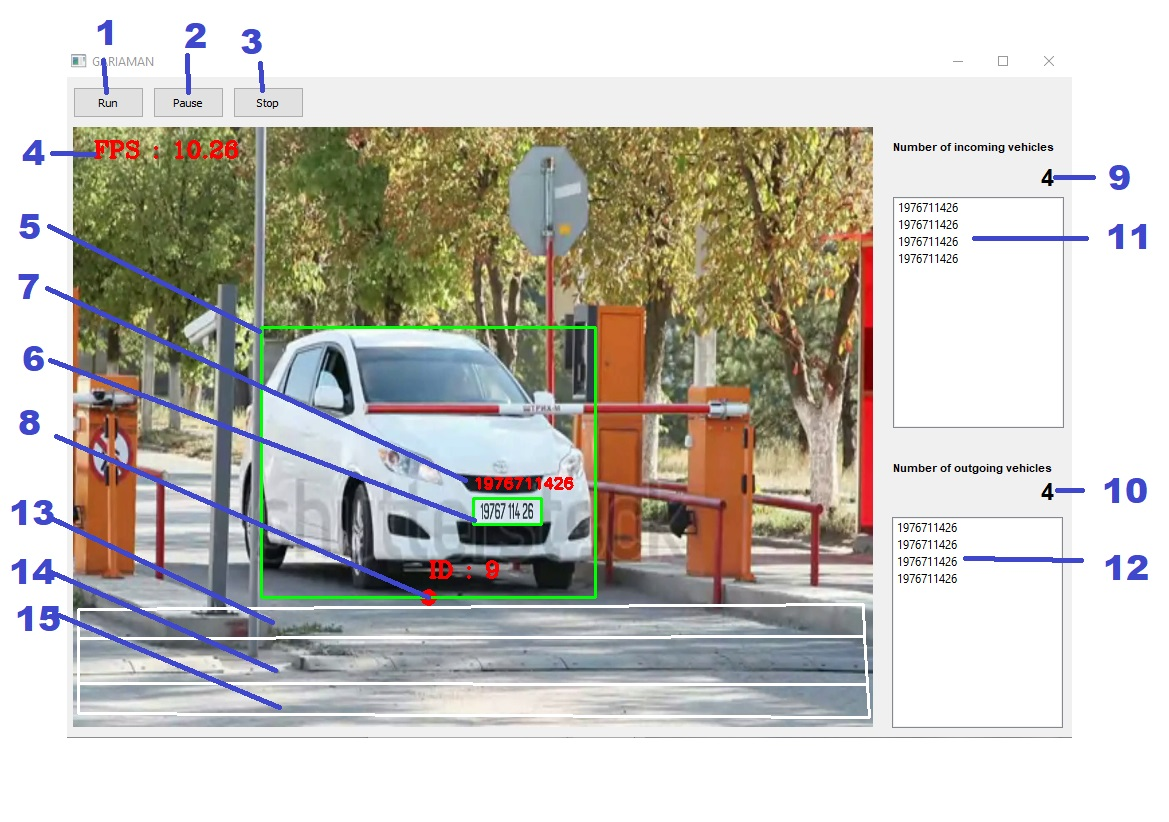
\includegraphics[height=10cm]{ch4-GARIAMAN-001.jpg}
	\caption{Interface graphique de l'application bureautique }
    \label{fig:final_soft}
\end{figure}
\begin{outline}
\1 1. Bouton de démarrage : permet de lancer la lecture de la vidéo à partir des caméras de surveillance.
\1 2. Bouton de pause : permet de figer la vidéo à un instant précis.
\1 3. Bouton d'arrêt : permet d'arrêter la lecture de la vidéo.
\1 4. Taux de rafraîchissement des images par seconde.
\1 5. Boite de délimitation indiquant le véhicule détecté.
\1 6. Boite de délimitation qui encadre la plaque d'immatriculation identifiée.
\1 7. Reconnaissance en temps réel les numéros de plaque d'immatriculation pour le véhicule détecté.
\1 8. Ligne de suivi virtuelle de la voiture avec son identifiant unique.
\1 9. Nombre de véhicule entrant dans le parking.
\1 10. Nombre de véhicule sortant du parking.
\1 11. Liste des numéros de plaques d'immatriculation des voitures entrant dans le parking.
\1 12. Liste des numéros de plaques d'immatriculation des véhicules sortant du parking.
\1 13, 14 et 15 : Ce sont des zones utilisées par l'algorithme de suivi qui a été expliqué dans la sous-section \ref{sec:traking}, où lorsque le point indiqué par la flèche 8 entre dans l'une des zones, le travail se fait comme suit :
       
    \2 Lorsque le point 8 est détecté dans la zone 13, puis quelque temps plus tard, il est détecté dans la zone 15 avec le même identifiant de voiture, le système conclut que la voiture est entrée dans le parking.

    \2 Lorsque le point 8 est détecté dans la zone 15, puis après un certain temps il est détecté dans la zone 13 avec le même identifiant de voiture, le système conclut que la voiture a quitté le parking.

    \2 Lors du passage du Point 8 à la Zone 14, la plaque d'immatriculation de ce véhicule est reconnue sur chaque photo (frame de vidéo ) et enregistrée dans la liste. Lorsque le point 8 quitte la zone 14, le numéro de plaque d'immatriculation le plus courant est envoyé à la base de données avec le statut \{ (Entrée) ou (Sortie) \}, puis la mémoire vive (RAM) sera libérée.
    
\1 Pour ajuster et modifier l'emplacement des zones de capteurs sur l'écran, qui sont constituées des zones 13, 14 et 15, il suffit de sélectionner la zone en cliquant avec le bouton droit de la souris.
   
\end{outline}

Après avoir effectué plusieurs étapes liées à la détection de véhicules, de plaques d'immatriculation et à la reconnaissance des chiffres d'immatriculation, ainsi que le suivi des véhicules, la vitesse de traitement des images a considérablement ralenti. La vitesse de traitement est passée à 10 images par seconde (FPS) en raison du temps nécessaire à la détection des véhicules (71 millisecondes), à la détection des chiffres sur la plaque d'immatriculation (20 millisecondes) et à d'autres tâches de traitement d'image et d'exécution de fonctions supplémentaires. En conséquence, le temps total d'exécution est désormais de 100 millisecondes par image. Pour résoudre ce problème de lenteur, nous envisageons de modifier les outils de développement de l'application  afin de le rendre plus rapide.

\section{Embarquement de l'application de gestion de parking sur les smartphones}

Afin de déployer l'application de gestion de parking pour les véhicules en Algérie sur des appareils mobiles et des puces intégrées, nous avons converti les fichiers de poids résultant de l'entraînement de l'algorithme YOLOV8 en un framework NCNN. Cette étape était essentielle car ces appareils ne prennent généralement pas en charge le langage Python, qui est également moins performant en raison de sa nature interprétée.

Ensuite, nous avons développé une application en \textbf{C++} pour tester et évaluer la vitesse de détection et de reconnaissance à la fois sur un ordinateur portable et un smartphone. Voici les résultats que nous avons obtenus :\\
Sur un ordinateur portable, nous avons atteint les valeurs de FPS suivantes :
\begin{outline}
    \1 27 FPS en utilisant le CPU,
    \1 17 FPS en utilisant le GPU.    
\end{outline}

En ce qui concerne le smartphone, nous avons obtenu les résultats suivants :
\begin{outline}
    \1 25 FPS en utilisant le CPU,
    \1 13 FPS en utilisant le GPU.
\end{outline}

Dans la figure \ref{fig:ch4-application_android}, une capture d'écran de l'interface de l'application mobile est affichée, montrant le résultat de détection de la voiture du test avec sa plaque d'immatriculation. Ce que nous avons remarqué est que la plaque d'immatriculation a été efficacement lue  malgré une vitesse de trame moyenne atteignant 25 images par seconde (FPS).


\begin{figure}[H]
	\centering
	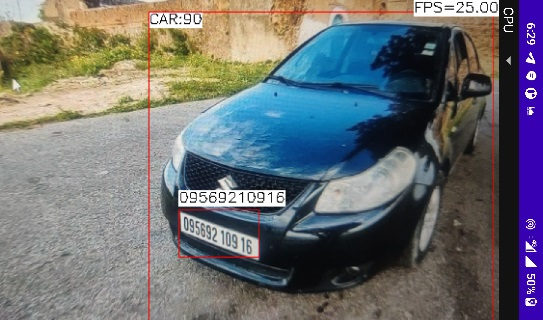
\includegraphics[height=5cm]{ch4-application_android.png}
	\caption{Capture d'écran de l'interface de l'application Android}
    \label{fig:ch4-application_android}
\end{figure}

Il est important de noter que sur un smartphone, la vitesse de rafraîchissement des images (frames) n'est pas constante. Cela est dû au fait que lorsque la température du processeur augmente, le téléphone réduit ses performances.

\section{Problèmes rencontrés et solution adoptées}

Lors du développement des différents modules de l'application, plusieurs problèmes ont été identifiés. Cette section présente les principaux problèmes techniques ainsi que les solutions adoptées.

\textbf{Problème 1:} Une difficulté persistante résidait dans la détection irrégulière des voitures par le modèle YOLO. Dans certaines images, le modèle détectait effectivement une voiture, mais cette détection échouait dans l'image suivante. Cette situation engendrait des interruptions dans la séquence des identifiants de suivi des voitures tout au long de la vidéo.

\textbf{Solution 1:}  Nous avons résolu ce problème en utilisant un filtre de Kalman pour chaque identifiant de voiture. Cette solution permet au système d'estimer la position de la voiture lorsque le détecteur YOLO ne parvient pas à la détecter.

\textbf{Problème 2:}  La lecture répétée des plaques d'immatriculation par notre système à chaque image de la vidéo peut entraîner la répétition de la reconnaissance (lecture) de la même plaque pour une seule voiture, avec parfois des erreurs de reconnaissance.

\textbf{Solution2: }  Pour remédier à cette situation, nous avons mis en place une solution consistant à créer une liste spécifique pour chaque identifiant de voiture. Dans cette liste, nous stockons toutes les plaques d'immatriculation lues pendant le mouvement de la voiture de la zone A à la zone B. Lorsque la voiture quitte la zone B, nous enregistrons les plaques d'immatriculation les plus fréquemment lues dans une base de données. Cette approche contribue à éviter les lectures répétées et à améliorer la fiabilité de la lecture des plaques d'immatriculation.

\section{Conclusion}

Dans ce dernier chapitre, nous avons décrit notre système de gestion de parking pour les véhicules en Algérie. Ce système est capable de détecter les véhicules, les plaques d'immatriculation, de reconnaître les chiffres d'immatriculation et de suivre le mouvement des véhicules entrant et sortant d'un parking. Il repose sur des techniques avancées de vision par ordinateur, en particulier l'apprentissage profond.

Nous avons évalué plusieurs algorithmes de détection d'objets, et à la suite de nombreuses expériences, nous avons choisi YOLOv8n en raison de ses performances exceptionnelles en matière de détection et de reconnaissance. Nous avons également testé divers outils OCR pour la lecture des plaques d'immatriculation. Les résultats obtenus ont montré la supériorité du modèle YOLOv8n dans cette tâche.

%%%%%%%%%%%%pour expliquer le processus de suivi de voiture et de plaque d'immatriculation tout au long de la vidéo, on assignent des identifiants uniques et on analysent leur mouvement pour déterminer leur entrée ou leur sortie du parking.

% Voici une explication générale des étapes mentionnées précédemment:

% \begin{outline}[enumerate]
%     \1 Réception de la vidéo a partir de la caméra de surveillance en temps réel :
%         \2 nous pouvons utiliser la bibliothèque OpenCV pour capturer la vidéo en temps réel à partir de la caméra de surveillance.

%     \1 Détection des voitures et des plaques d'immatriculation à l'aide d'un modèle de détection d'objets :
%        \2 nous pouvons utiliser des modèles tels que Faster R-CNN ou SSD Mobile net v3  ou YOLOV8 pour détecter les voitures dans les images vidéo.
    
%     \1 Découpage de la partie d'image contenant la plaque d'immatriculation :
%        \2 Une fois les voitures et les plaques d'immatriculation détectées, nous pouvons découper la partie de l'image qui contient la plaque d'immatriculation.  en utilisant des bibliothèques de traitement d'image comme OpenCV.
    
%     \1 Extraction du texte (de la plaque d'immatriculation):
%        \2 Pour lire la plaque d'immatriculation, nous pouvons utiliser des algorithmes OCR ou développer un algorithme personnalisé.
    
%     \1 Suivi des voitures dans une vidéo:
%        \2 Il existe plusieurs algorithmes de suivi d'objets que nous pouvons utiliser pour suivre le mouvement des voitures entre les images vidéo consécutives , mais celui qui peut être utilisé dans notre projet est l'algorithme de détection et de suivi (Detection and Tracking) .
    
%     \1 Attribution d'identifiants aux voitures :
%        \2 Lors du suivi des voitures, nous attribuons un identifiant unique à chaque voiture dans la scène, ainsi qu'à sa plaque d'immatriculation.
    
%     \1 Analyse du mouvement des voitures pour déterminer si elles entrent ou sortent du parking :
%        \2 Nous utilisons les identifiants attribués pour analyser le mouvement des voitures, déterminer leur direction et savoir si elles entrent ou sortent du parking.
    
%     \1 Détermination du nombre de voitures entrantes et sortantes du parking :
%         \2 Calcule du nombre de voitures entrantes et sortantes du parking en fonction de l'analyse du mouvement des voitures qui a été effectuée
       
% \end{outline}

% %%%%%%%%%%%%%%%%%%%
% Pour entraîner un modèle de détection d'objets dans des images, plusieurs étapes importantes doivent généralement être suivies:
% \begin{outline}[enumerate]
%     \1 Chargement des bibliothèques : Commençons par charger les bibliothèques de base telles que PyTorch et TorchVision.

%     \1 Sélection et personnalisation du modèle : Choisissons le modèle que nous souhaitons entraîner et personnalisons ses paramètres de base tels que la forme des entrées et des sorties, ainsi que d'autres paramètres selon nos besoins.

%     \1 Création d'une classe pour la lecture des données : Écrivons une classe personnalisée pour lire l'ensemble de données composé d'images et de fichiers de annotations sur les objets, puis convertissons ces données en tensors compréhensibles par le framework.

%     \1 Préparation de données : Au sein de cette étape, redimensionnons les images pour les adapter aux exigences du modèle de détection d'objets et assurons-nous que les données sont correctement formatées, notamment en effectuant le redimensionnement, la normalisation, et l'ajustement des dimensions au besoin.

%     \1 Chargement du modèle : Assurons-nous que le modèle est correctement chargé et converti dans un format compréhensible par le processeur graphique GPU ou l'unité centrale de traitement (CPU).

%     \1 Définition de la fonction de perte : Définissons et choisissons la fonction de perte appropriée à notre tâche .

%     \1 Sélection de l'optimiseur : Choisissons l'optimiseur à utiliser, tel que le SGD (Stochastic Gradient Descent), et configurons ses paramètres, y compris le taux d'apprentissage et le nombre d'étapes.

%     \1 Entraînement du modèle : Effectuons le processus d'entraînement en utilisant une boucle itérative qui comprend les étapes suivantes :
%    \2 Réinitialisation des gradients.
%    \2 Passage en avant (Forward Pass) pour obtenir les prédictions du modèle.
%    \2 Calcul de la perte entre les prédictions et les valeurs réelles.
%    \2 Rétropropagation (Backward Pass) et mise à jour des paramètres du modèle.

%    \1 Sauvegarde du modèle : Après l'entraînement, sauvegardons le modèle pour une utilisation ultérieure sans avoir besoin de le ré-entraîner.

%    \1 Évaluation du modèle : Évaluons les performances du modèle en utilisant des données de test ou de validation pour mesurer son efficacité.

%    \1 Utilisation du modèle : Après avoir réussi l'entraînement, nous pouvons utiliser le modèle pour détecter des objets dans de nouvelles images.

% \end{outline}